\chapter{Introdução}

Um dos papéis da engenharia de software é fornecer métodos, modelos e técnicas para que o software atenda às necessidades dos interessados em sua construção. A utilização desse conhecimento leva a uma forma aproximadamente ideal de realizar as atividades necessárias para o desenvolvimento do software. Os resultados  gerados por atividades realizadas dessa forma apresentarão um grau de qualidade elevado. Entretanto, essa forma ideal de realizar as atividades pode exigir recursos incompatíveis com os disponíveis para o projeto. Por esse motivo, as pessoas envolvidas com o projeto do software tendem a realizar essas atividades de modo que atendam às restrições de recursos e, ao mesmo tempo, estejam o mais próximas possíveis da maneira ideal. Entretanto, a existência de restrições de recursos demasiadamente severas faz com que algumas atividades tenham de ser realizadas de uma forma distante da ideal. Quando isso ocorre, é criada uma dívida técnica.




O termo dívida técnica é, na verdade, uma metáfora extraída da área financeira. Realizar uma atividade de forma não ideal é como adquirir uma dívida para com a qualidade do sistema.  Essa metáfora foi usada pela primeira vez por Cunningham\cite{cunningham1993wycash}. Ele percebeu que criar porções de código que não estivessem de acordo com as boas práticas da programação é semelhante a contrair uma dívida para com o sistema. Assim como na área financeira, essas dívidas causam o pagamento de juros. Esses juros são todas as dificuldades adicionais necessárias para manipular as porções de código feitas de forma incompatível com as boas práticas. 

Desde a criação do conceito por Cunningham\cite{cunningham1993wycash}, as dívidas técnicas têm atraído a atenção da comunidade científica.  Como pode ser visto na Figura \ref{fig:cap1_citacoes_td_ano}, houve um acréscimo de citações em trabalhos acadêmicos. 


  \begin{figure}[H]
  \centering
  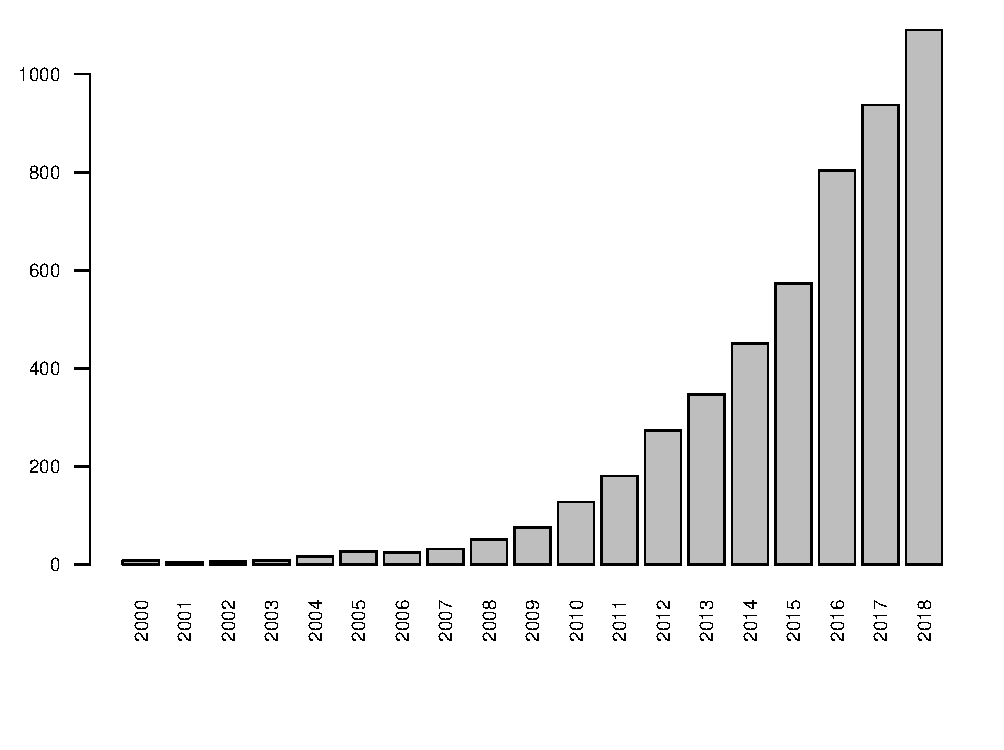
\includegraphics{capitulo_introducao/numero_citacoes.pdf} 
  \caption{Número anual de citações ao termo dívida técnica em trabalhos científicos. }
  \label{fig:cap1_citacoes_td_ano} 
\end{figure}


Neste trabalho, proporemos um modelo para estimar os juros da dívida técnica em projetos de software. Esse modelo considerará os juros como a diminuição, causada pela existência da dívida técnica, da produtividade nos projetos. O modelo proposto será analisado por meio de um estudo de caso envolvendo 1814 projetos de software livre.


\section{Motivação}

Embora a existência de dívidas técnicas traga consequências ruins para a evolução do software, nem sempre elas são algo totalmente negativo. Muitas vezes, adquirir uma dívida técnica é a opção mais correta para que haja um ganho de velocidade e não se perca uma oportunidade de negócio por exemplo.  Apesar disso, a aquisição de dívidas técnicas não pode ser feita descontroladamente. É necessário que haja um gerenciamento para mantê-la em patamares aceitáveis.  Caso o seu nível atinja um patamar muito alto, é possível que os juros causados por ela inviabilizem todo o processo de desenvolvimento e evolução do software. Essa inviabilidade se concretiza quando o esforço necessário para inserir novas funcionalidades é maior do que os benefícios trazidos por essas funcionalidades.

O gerenciamento da dívida técnica é baseado em duas informações:
\begin{itemize}
\item[(i)] O esforço necessário para corrigir uma dívida técnica. Essa informação é denominada como o \textbf{principal} da dívida técnica.
\item[(ii)] O esforço adicional necessário para realizar as futuras atividades de desenvolvimento, evolução e manutenção do software.  Esse esforço adicional é chamado de \textbf{juros} da dívida técnica.
\end{itemize}

Dentre esses dois elementos, existe uma necessidade especial em gerenciar os juros da dívida técnica. Isso acontece pois \textbf{os juros são aquilo que efetivamente influenciam negativamente os projetos de software}.  O que faz com que seja necessário alocar recursos para quitar uma dívida técnica é o quanto de \textbf{juros} essa dívida está gerando.  Ou seja, o quanto ela está influenciando negativamente o desenvolvimento e manutenção do sistema.   À medida que os juros crescem inadvertidamente,  cada vez mais atividades são realizadas apenas para estabilizar o software em vez de adicionar funcionalidades e melhorias. Em certos casos, inclusive, é cogitado o descarte do software atual a fim de que uma nova versão seja produzida do início \cite{sterling2010managing}. Dessa forma, obter estimativas a respeito dos juros é uma atividade essencial do gerenciamento da dívida técnica. 

\section{Dificuldades na estimação dos juros da dívida técnica}


O problema de estimar os juros é um dos mais difíceis dentro do espectro de problemas encontrados na área do gerenciamento da dívida técnica.\cite{zazworka2011investigating,power2013understanding,yli2016software,schmid2013formal}. Elencamos dois dos fatores que acreditamos serem os maiores responsáveis por essa dificuldade:

\begin{enumerate}


\item \textbf{A incidência ou não dos juros depende de eventos que ocorrerão no futuro.} Um exemplo é a existência de uma dívida técnica em um trecho do código que poderá ou não ser alterado no futuro. Se ele não for, então não haverá juros já que não haverá uma dificuldade extra para alterá-lo. Prever a ocorrência desses eventos é uma tarefa difícil e até mesmo impossível em algumas situações.

\item \textbf{Necessidade de uma análise ampla a respeito dos impactos dos juros.} Os juros podem impactar diversos aspectos do desenvolvimento de um software. Algumas desses impactos podem ser em aspectos mais técnicos, como a dificuldade em adicionar novas funcionalidades devido à inexistência de testes automatizados, ou menos técnicos, como a motivação  e a moral da equipe\cite{spinola2013investigating}.
Dessa forma, uma abordagem plenamente eficaz  para a estimação dos juros da dívida técnica deverá conseguir capturar esses variados impactos de uma forma ampla e que considere o contexto no qual eles ocorrem.




\end{enumerate}


\section{Propostas atuais}
\label{modelos_existentes}

São encontradas na literatura poucas propostas de estratégias para calcular os juros da dívida técnica.  Isso fica evidente quando são analisadas alguns dos mapeamentos sistemáticos realizados na área\cite{ampatzoglou2015financial,li2015systematic,behutiye2017analyzing}. Apesar da relevância e qualidade dos trabalhos existentes, podemos citar alguns pontos que nos levam a acreditar que o problema da estimação dos juros da dívida técnica ainda não foi totalmente resolvido:

\begin{itemize}
\item \textbf{Não há uma consenso a respeito de como expressar os juros de um software}. Singh et al.\cite{singh2014framework} define os juros como o tempo extra utilizado para compreender o código. Enquanto isso, Nugroho et al.\cite{nugroho2011empirical} e Ampatzoglou et al. \cite{ampatzoglou2015financial,ampatzoglou2018framework} consideram os juros como o esforço extra de manutenção causado pela existência da dívida técnica. Por fim, Falessi. et al. \cite{falessi2015towards} define os juros da dívida técnica como a quantidade adicional de defeitos do software.
\item \textbf{Nenhuma das propostas encontradas foi avaliada usando dados de um número grande de projetos.} Todas as propostas atuais para a estimação dos juros da dívida técnica foram validadas utilizando um conjunto muito limitado de projetos. Alguns exemplos são os trabalhos de Singh et al.\cite{singh2014framework} e Nugroho et al. \cite{nugroho2011empirical} que validam suas propostas utilizando dados de apenas um projeto. Acreditamos que seja necessário incluir um número de projetos maior no processo de validação de uma estratégia para estimação dos juros da dívida técnica. 

\end{itemize}

Além da escassez de estudos sobre o cálculo dos juros da dívida técnica, existe uma falta ainda maior de trabalhos quantitativos. Conforme argumentado por Brown, N et al.\cite{brown2010managing}, há uma predominância na utilização de métodos qualitativos nas pesquisas a respeito da dívida técnica e isso pode levar a conclusões baseadas em intuições atraentes, porém não necessariamente corretas. Essas conclusões incorretas podem ser explicadas pela existência de dados obtidos por meio de declarações imprecisas. Essa imprecisão pode ser causada pela dificuldade que as pessoas envolvidas com os projetos de software têm em assumir suas deficiências ou falhas. Por isso, Brown, N et al.\cite{brown2010managing} indica a necessidade da criação de modelos baseados em abordagens quantitativas para viabilizar a criação de rigorosas técnicas de gerenciamento da dívida técnica que possam ser aplicadas em projetos de larga escala. 


\section{O modelo de estimação}


Nossa hipótese é que todas as formas existentes de expressar os juros da dívida técnica de um projeto podem ser unificadas em apenas uma: \emph{Os juros da dívida técnica são a diminuição, causada pela existência da dívida técnica, da produtividade do projeto}.  Essa hipótese será aplicada em um modelo que será utilizado para estimar os juros da dívida técnica. O funcionamento básico desse modelo pode ser descrito em três passos:

\begin{enumerate}
\item Definimos um grupo $G$ de projetos que sejam todos semelhantes entre si.
\item Dividimos o grupo $G$ em duas partições: 
\begin{enumerate}
\item[$P_1$] Projetos com pouca dívida técnica.
\item[$P_2$] Projetos com muita dívida técnica.
\end{enumerate}
\item Estimamos os juros da dívida técnica dos projetos na partição $P_2$ como a diferença média da produtividade média dos projetos em $P_1$ menos a produtividade média dos projetos em $P_2$.
\end{enumerate}


Evidentemente, existem diversas dificuldades de realizar a estimação dos juros da dívida técnica utilizando esse modelo. Algumas delas são:

\begin{itemize}
\item Como determinar o grau de semelhança entre dois projetos.
\item Como calcular a produtividade dos projetos.
\item Como definir se um projeto tem muita ou pouca dívida técnica.
\end{itemize}

No decorrer desta pesquisa, descreveremos e testaremos algumas soluções para essas dificuldades apresentadas. Além disso, o modelo proposto será avaliado utilizando dados de 1814 projetos de software livre.


\section{Objetivos}
Os principais objetivos desta pesquisa são os seguintes:

\begin{itemize}
\item  \textbf{Propor um modelo quantitativo para estimar os juros da dívida técnica.} Devido à escassez de trabalhos quantitativos e empiricamente avaliados, acreditamos que, por meio desse modelo, haverá uma contribuição para a resolução do problema de estimação dos juros da dívida técnica. O modelo que será proposto é baseado na comparação da produtividade dos projetos quando eles são realizados em dois cenários diferentes: um com dívida técnica e outro ``sem dívida técnica". Temos como hipótese que haverá uma diminuição da produtividade quando há a existência de dívidas. Essa diminuição é, na verdade, os juros da dívida técnica. Conforme veremos na seção \ref{modelos_existentes}, outros modelos também propõem uma abordagem de estimação dos juros comparando dois cenários. Porém, nenhum deles considera a produtividade nessa comparação. 
\item  \textbf{Avaliar a utilização desse modelo em um estudo de caso envolvendo um grande número de projetos de software livre.} Apesar de poucos, existem alguns modelos para estimação dos juros. Porém, até onde vai o nosso conhecimento, nenhum deles foi submetido a uma avaliação utilizando uma quantidade significativa de projetos. Nesta pesquisa iremos utilizar o modelo de estimação proposto para avaliar 1814 projetos de software livre.
\item  \textbf{Aumentar a precisão do gerenciamento da dívida técnica.}  Possibilitando que as pessoas possam ter uma estimativa de quanto juros serão pagos para as dívidas, elas poderão decidir melhor quais dívidas devem ou não ser adquiridas e principalmente qual o nível de dívida técnica é aceitável de acordo com suas necessidades. 
\end{itemize}


\section{Resumo deste trabalho}
A Figura \ref{fig:resumo_geral_pesquisa} apresenta um resumo deste trabalho. Inicialmente apresentamos uma revisão com os principais conceitos relacionados às dívidas técnicas e, em particular, a relevância do problema de estimação dos juros da dívida técnica. Em seguida apresentamos nosso modelo abstrato de estimação dos juros e uma instância específica para o contexto dos software livres. Por fim, apresentamos um estudo de caso múltiplo onde esse modelo é avaliado. 



 \begin{figure}[H]
  \centering
  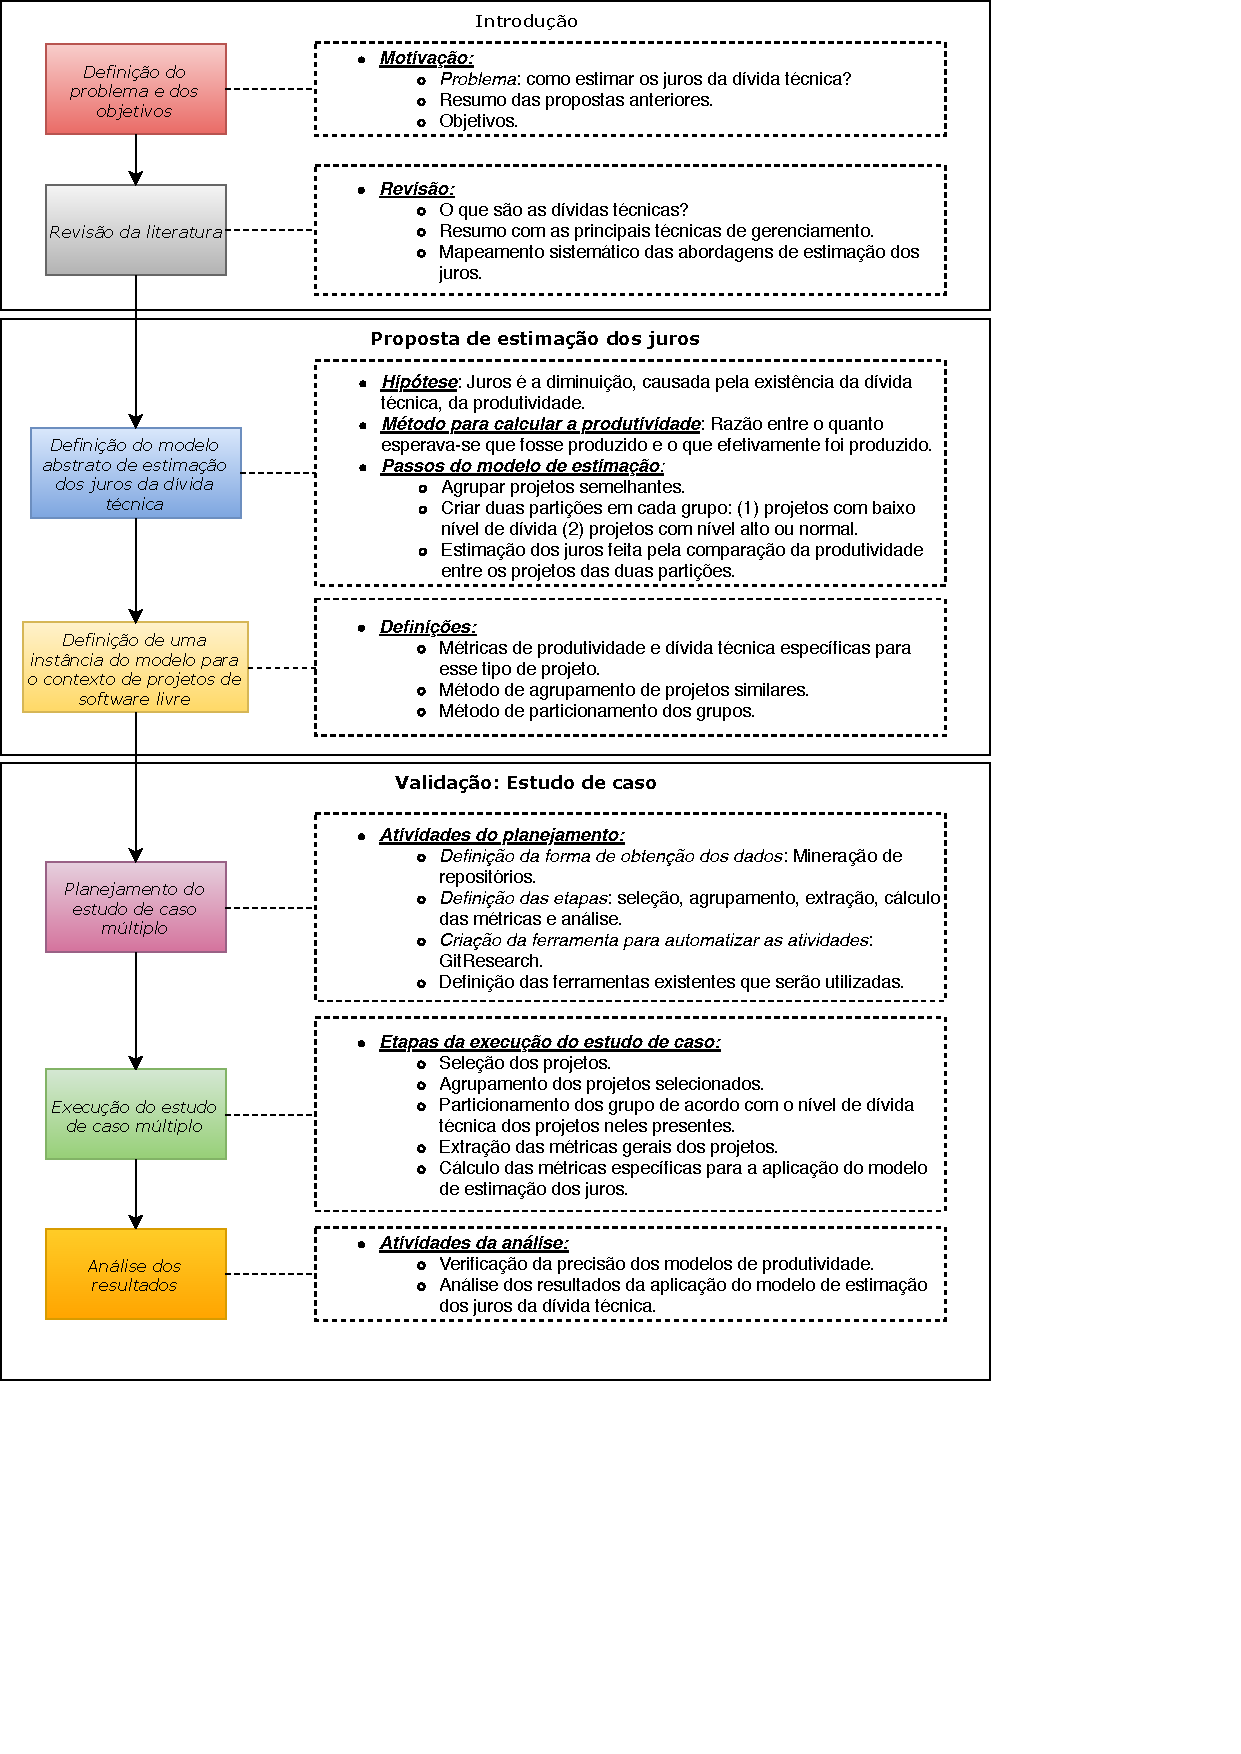
\includegraphics[trim={0cm 6cm 0cm 0cm},clip]{capitulo_introducao/resumo_geral_pesquisa.pdf}
  \caption{Resumo das atividades desta pesquisa.}
  \label{fig:resumo_geral_pesquisa} 
\end{figure}










\section{Organização do texto}

O restante deste texto é organizado da seguinte forma. No Capítulo 2 descrevemos a dívida técnica. São apresentadas as formas de classificação encontradas na literatura e os diversos tipos de dívida técnica. No Capítulo 3 propomos um modelo abstrato de estimação dos juros da dívida técnica e no Capítulo 4 apresentamos uma instância desse modelo específica para o contexto dos softwares livres.  No Capítulo 5 realizamos o planejamento de um estudo de caso para validar o modelo  proposto. No Capítulo 6 descrevemos os detalhes a respeito da execução do estudo de caso e os resultados obtidos.  No Capítulo 7 concluímos o trabalho descrevendo os principais resultados. Por fim, fornecemos as referências bibliográficas que utilizamos para a realização desta pesquisa.






























